
%% bare_conf.tex
%% V1.4b
%% 2015/08/26
%% by Michael Shell
%% See:
%% http://www.michaelshell.org/
%% for current contact information.
%%
%% This is a skeleton file demonstrating the use of IEEEtran.cls
%% (requires IEEEtran.cls version 1.8b or later) with an IEEE
%% conference paper.
%%
%% Support sites:
%% http://www.michaelshell.org/tex/ieeetran/
%% http://www.ctan.org/pkg/ieeetran
%% and
%% http://www.ieee.org/

%%*************************************************************************
%% Legal Notice:
%% This code is offered as-is without any warranty either expressed or
%% implied; without even the implied warranty of MERCHANTABILITY or
%% FITNESS FOR A PARTICULAR PURPOSE!
%% User assumes all risk.
%% In no event shall the IEEE or any contributor to this code be liable for
%% any damages or losses, including, but not limited to, incidental,
%% consequential, or any other damages, resulting from the use or misuse
%% of any information contained here.
%%
%% All comments are the opinions of their respective authors and are not
%% necessarily endorsed by the IEEE.
%%
%% This work is distributed under the LaTeX Project Public License (LPPL)
%% ( http://www.latex-project.org/ ) version 1.3, and may be freely used,
%% distributed and modified. A copy of the LPPL, version 1.3, is included
%% in the base LaTeX documentation of all distributions of LaTeX released
%% 2003/12/01 or later.
%% Retain all contribution notices and credits.
%% ** Modified files should be clearly indicated as such, including  **
%% ** renaming them and changing author support contact information. **
%%*************************************************************************


% *** Authors should verify (and, if needed, correct) their LaTeX system  ***
% *** with the testflow diagnostic prior to trusting their LaTeX platform ***
% *** with production work. The IEEE's font choices and paper sizes can   ***
% *** trigger bugs that do not appear when using other class files.       ***                          ***
% The testflow support page is at:
% http://www.michaelshell.org/tex/testflow/



\documentclass[conference]{IEEEtran}
% Some Computer Society conferences also require the compsoc mode option,
% but others use the standard conference format.
%
% If IEEEtran.cls has not been installed into the LaTeX system files,
% manually specify the path to it like:
% \documentclass[conference]{../sty/IEEEtran}





% Some very useful LaTeX packages include:
% (uncomment the ones you want to load)


% *** MISC UTILITY PACKAGES ***
%
%\usepackage{ifpdf}
% Heiko Oberdiek's ifpdf.sty is very useful if you need conditional
% compilation based on whether the output is pdf or dvi.
% usage:
% \ifpdf
%   % pdf code
% \else
%   % dvi code
% \fi
% The latest version of ifpdf.sty can be obtained from:
% http://www.ctan.org/pkg/ifpdf
% Also, note that IEEEtran.cls V1.7 and later provides a builtin
% \ifCLASSINFOpdf conditional that works the same way.
% When switching from latex to pdflatex and vice-versa, the compiler may
% have to be run twice to clear warning/error messages.






% *** CITATION PACKAGES ***
%
%\usepackage{cite}
% cite.sty was written by Donald Arseneau
% V1.6 and later of IEEEtran pre-defines the format of the cite.sty package
% \cite{} output to follow that of the IEEE. Loading the cite package will
% result in citation numbers being automatically sorted and properly
% "compressed/ranged". e.g., [1], \cite{seznec2007tage}, \cite{calder1997evidence}, \cite{lee1995branch}, \cite{jimenez2001dynamic}, \cite{jimenez2003fast} without using
% cite.sty will become [1], \cite{calder1997evidence}, \cite{jimenez2001dynamic}--\cite{lee1995branch}, \cite{seznec2007tage} using cite.sty. cite.sty's
% \cite will automatically add leading space, if needed. Use cite.sty's
% noadjust option (cite.sty V3.8 and later) if you want to turn this off
% such as if a citation ever needs to be enclosed in parenthesis.
% cite.sty is already installed on most LaTeX systems. Be sure and use
% version 5.0 (2009-03-20) and later if using hyperref.sty.
% The latest version can be obtained at:
% http://www.ctan.org/pkg/cite
% The documentation is contained in the cite.sty file itself.






% *** GRAPHICS RELATED PACKAGES ***
%
\ifCLASSINFOpdf
  % \usepackage[pdftex]{graphicx}
  % declare the path(s) where your graphic files are
  % \graphicspath{{../pdf/}{../jpeg/}}
  % and their extensions so you won't have to specify these with
  % every instance of \includegraphics
  % \DeclareGraphicsExtensions{.pdf,.jpeg,.png}
\else
  % or other class option (dvipsone, dvipdf, if not using dvips). graphicx
  % will default to the driver specified in the system graphics.cfg if no
  % driver is specified.
  % \usepackage[dvips]{graphicx}
  % declare the path(s) where your graphic files are
  % \graphicspath{{../eps/}}
  % and their extensions so you won't have to specify these with
  % every instance of \includegraphics
  % \DeclareGraphicsExtensions{.eps}
\fi
\usepackage{algorithm}
\usepackage{algpseudocode}
\usepackage{amsmath}
\usepackage{amsmath,amssymb,amsthm,latexsym,paralist, booktabs}
\usepackage{url}
\usepackage[pdftex]{graphicx}
% default pic path
\usepackage{bm}
\usepackage{mathtools}
\let\oldvec\vec
\renewcommand{\vec}[1]{\oldvec{\mathit{#1}}}
\newcommand{\mat}[1]{\mathbf{#1}} % undergraduate algebra version
\newcommand{\parallelsum}{\mathbin{\!/\mkern-5mu/\!}}
\graphicspath{{pics/}}
\usepackage{subfigure}

\usepackage{listings}
\usepackage{color} %red, green, blue, yellow, cyan, magenta, black, white
\definecolor{mygreen}{RGB}{28,172,0} % color values Red, Green, Blue
\definecolor{mylilas}{RGB}{170,55,241}

%\newcommand{\mat}[1]{\bm{\mathit{#1}}}




% *** Do not adjust lengths that control margins, column widths, etc. ***
% *** Do not use packages that alter fonts (such as pslatex).         ***
% There should be no need to do such things with IEEEtran.cls V1.6 and later.
% (Unless specifically asked to do so by the journal or conference you plan
% to submit to, of course. )


% correct bad hyphenation here
\hyphenation{op-tical net-works semi-conduc-tor}


\begin{document}
\lstset{language=Matlab,%
    %basicstyle=\color{red},
    breaklines=true,%
    morekeywords={matlab2tikz},
    keywordstyle=\color{blue},%
    morekeywords=[2]{1}, keywordstyle=[2]{\color{black}},
    identifierstyle=\color{black},%
    stringstyle=\color{mylilas},
    commentstyle=\color{mygreen},%
    showstringspaces=false,%without this there will be a symbol in the places where there is a space
    numbers=left,%
    numberstyle={\tiny \color{black}},% size of the numbers
    numbersep=9pt, % this defines how far the numbers are from the text
    emph=[1]{for,end,break},emphstyle=[1]\color{red}, %some words to emphasise
    %emph=[2]{word1,word2}, emphstyle=[2]{style},    
}
%
% paper title
% Titles are generally capitalized except for words such as a, an, and, as,
% at, but, by, for, in, nor, of, on, or, the, to and up, which are usually
% not capitalized unless they are the first or last word of the title.
% Linebreaks \\ can be used within to get better formatting as desired.
% Do not put math or special symbols in the title.
\title{CSCE 643 Multi-View Geometry CV\\
Project II}


% author names and affiliations
% use a multiple column layout for up to three different
% affiliations

% conference papers do not typically use \thanks and this command
% is locked out in conference mode. If really needed, such as for
% the acknowledgment of grants, issue a \IEEEoverridecommandlockouts
% after \documentclass

% for over three affiliations, or if they all won't fit within the width
% of the page, use this alternative format:
%
%\author{\IEEEauthorblockN{Michael Shell\IEEEauthorrefmark{1},
%Homer Simpson\IEEEauthorrefmark{2},
%James Kirk\IEEEauthorrefmark{3},
%Montgomery Scott\IEEEauthorrefmark{3} and
%Eldon Tyrell\IEEEauthorrefmark{4}}
%\IEEEauthorblockA{\IEEEauthorrefmark{1}School of Electrical and Computer Engineering\\
%Georgia Institute of Technology,
%Atlanta, Georgia 30332--0250\\ Email: see http://www.michaelshell.org/contact.html}
%\IEEEauthorblockA{\IEEEauthorrefmark{2}Twentieth Century Fox, Springfield, USA\\
%Email: homer@thesimpsons.com}
%\IEEEauthorblockA{\IEEEauthorrefmark{3}Starfleet Academy, San Francisco, California 96678-2391\\
%Telephone: (800) 555--1212, Fax: (888) 555--1212}
%\IEEEauthorblockA{\IEEEauthorrefmark{4}Tyrell Inc., 123 Replicant Street, Los Angeles, California 90210--4321}}




% use for special paper notices
%\IEEEspecialpapernotice{(Invited Paper)}




% make the title area
\maketitle
\begin{abstract}
In this project, we explore and investigate different approaches for estimation in 2D projective transformation. In total, we implemented 3 approaches for finding the homography transformation between two different images, Direct Linear Transformation (DLT), normalized DLT and DLT with Sampson error minimization. This paper mainly focuses on the mathematical foundations for those methodologies used in our implementation and presents the results through combining two images into one panorama to validate the correctness of our approach. We can see clearly that with the advancement of our approach, the sampson error is gradually reduced (though there are few differences we can notice between those image panorama results).
\end{abstract}
% As a general rule, do not put math, special symbols or citations
% in the abstract

% no keywords




% For peer review papers, you can put extra information on the cover
% page as needed:
% \ifCLASSOPTIONpeerreview
% \begin{center} \bfseries EDICS Category: 3-BBND \end{center}
% \fi
%
% For peerreview papers, this IEEEtran command inserts a page break and
% creates the second title. It will be ignored for other modes.
\IEEEpeerreviewmaketitle


\section{Problem Formulation}
As shown in the project requirement documents, the aim of all problems in our project is to find a homography that can transform one image (shown in Fig. \ref{org_img} (a)) into the same space of another image (shown in Fig. \ref{org_img} (b)). Clearly, to achieve that, we have some points in common (basically overlappings) between those images as information we need to compute the homography. Suppose we have two set of points $\mat{x}_i$ and $\mat{x}_i^\prime$, which as mentioned are distributed in the overlapping portion of two images, the aim of this project is to use different approaches to compute the transformation homography $\mat{H}$ so that
\begin{equation}
	\mat{x}_i^\prime = \mat{H}\mat{x}_i
\end{equation}
in homogeneous space. Also be noticed that to acquire a better algorithm performance, those point pairs should be selected as accurate as possible and we should avoid choosing points that are colinear, coplanar, etc. Furthermore, in problem 3, we need to use sampson error and MLE methodologies to calculate the error of our homography and minimize the error to acquire better homography. The rest of this paper will be organized problem by problem.

\begin{figure*}[!hbpt]
  \subfigure[Original source image(the image we wanna transform)]{
\label{fig1} %% label for second subfigure
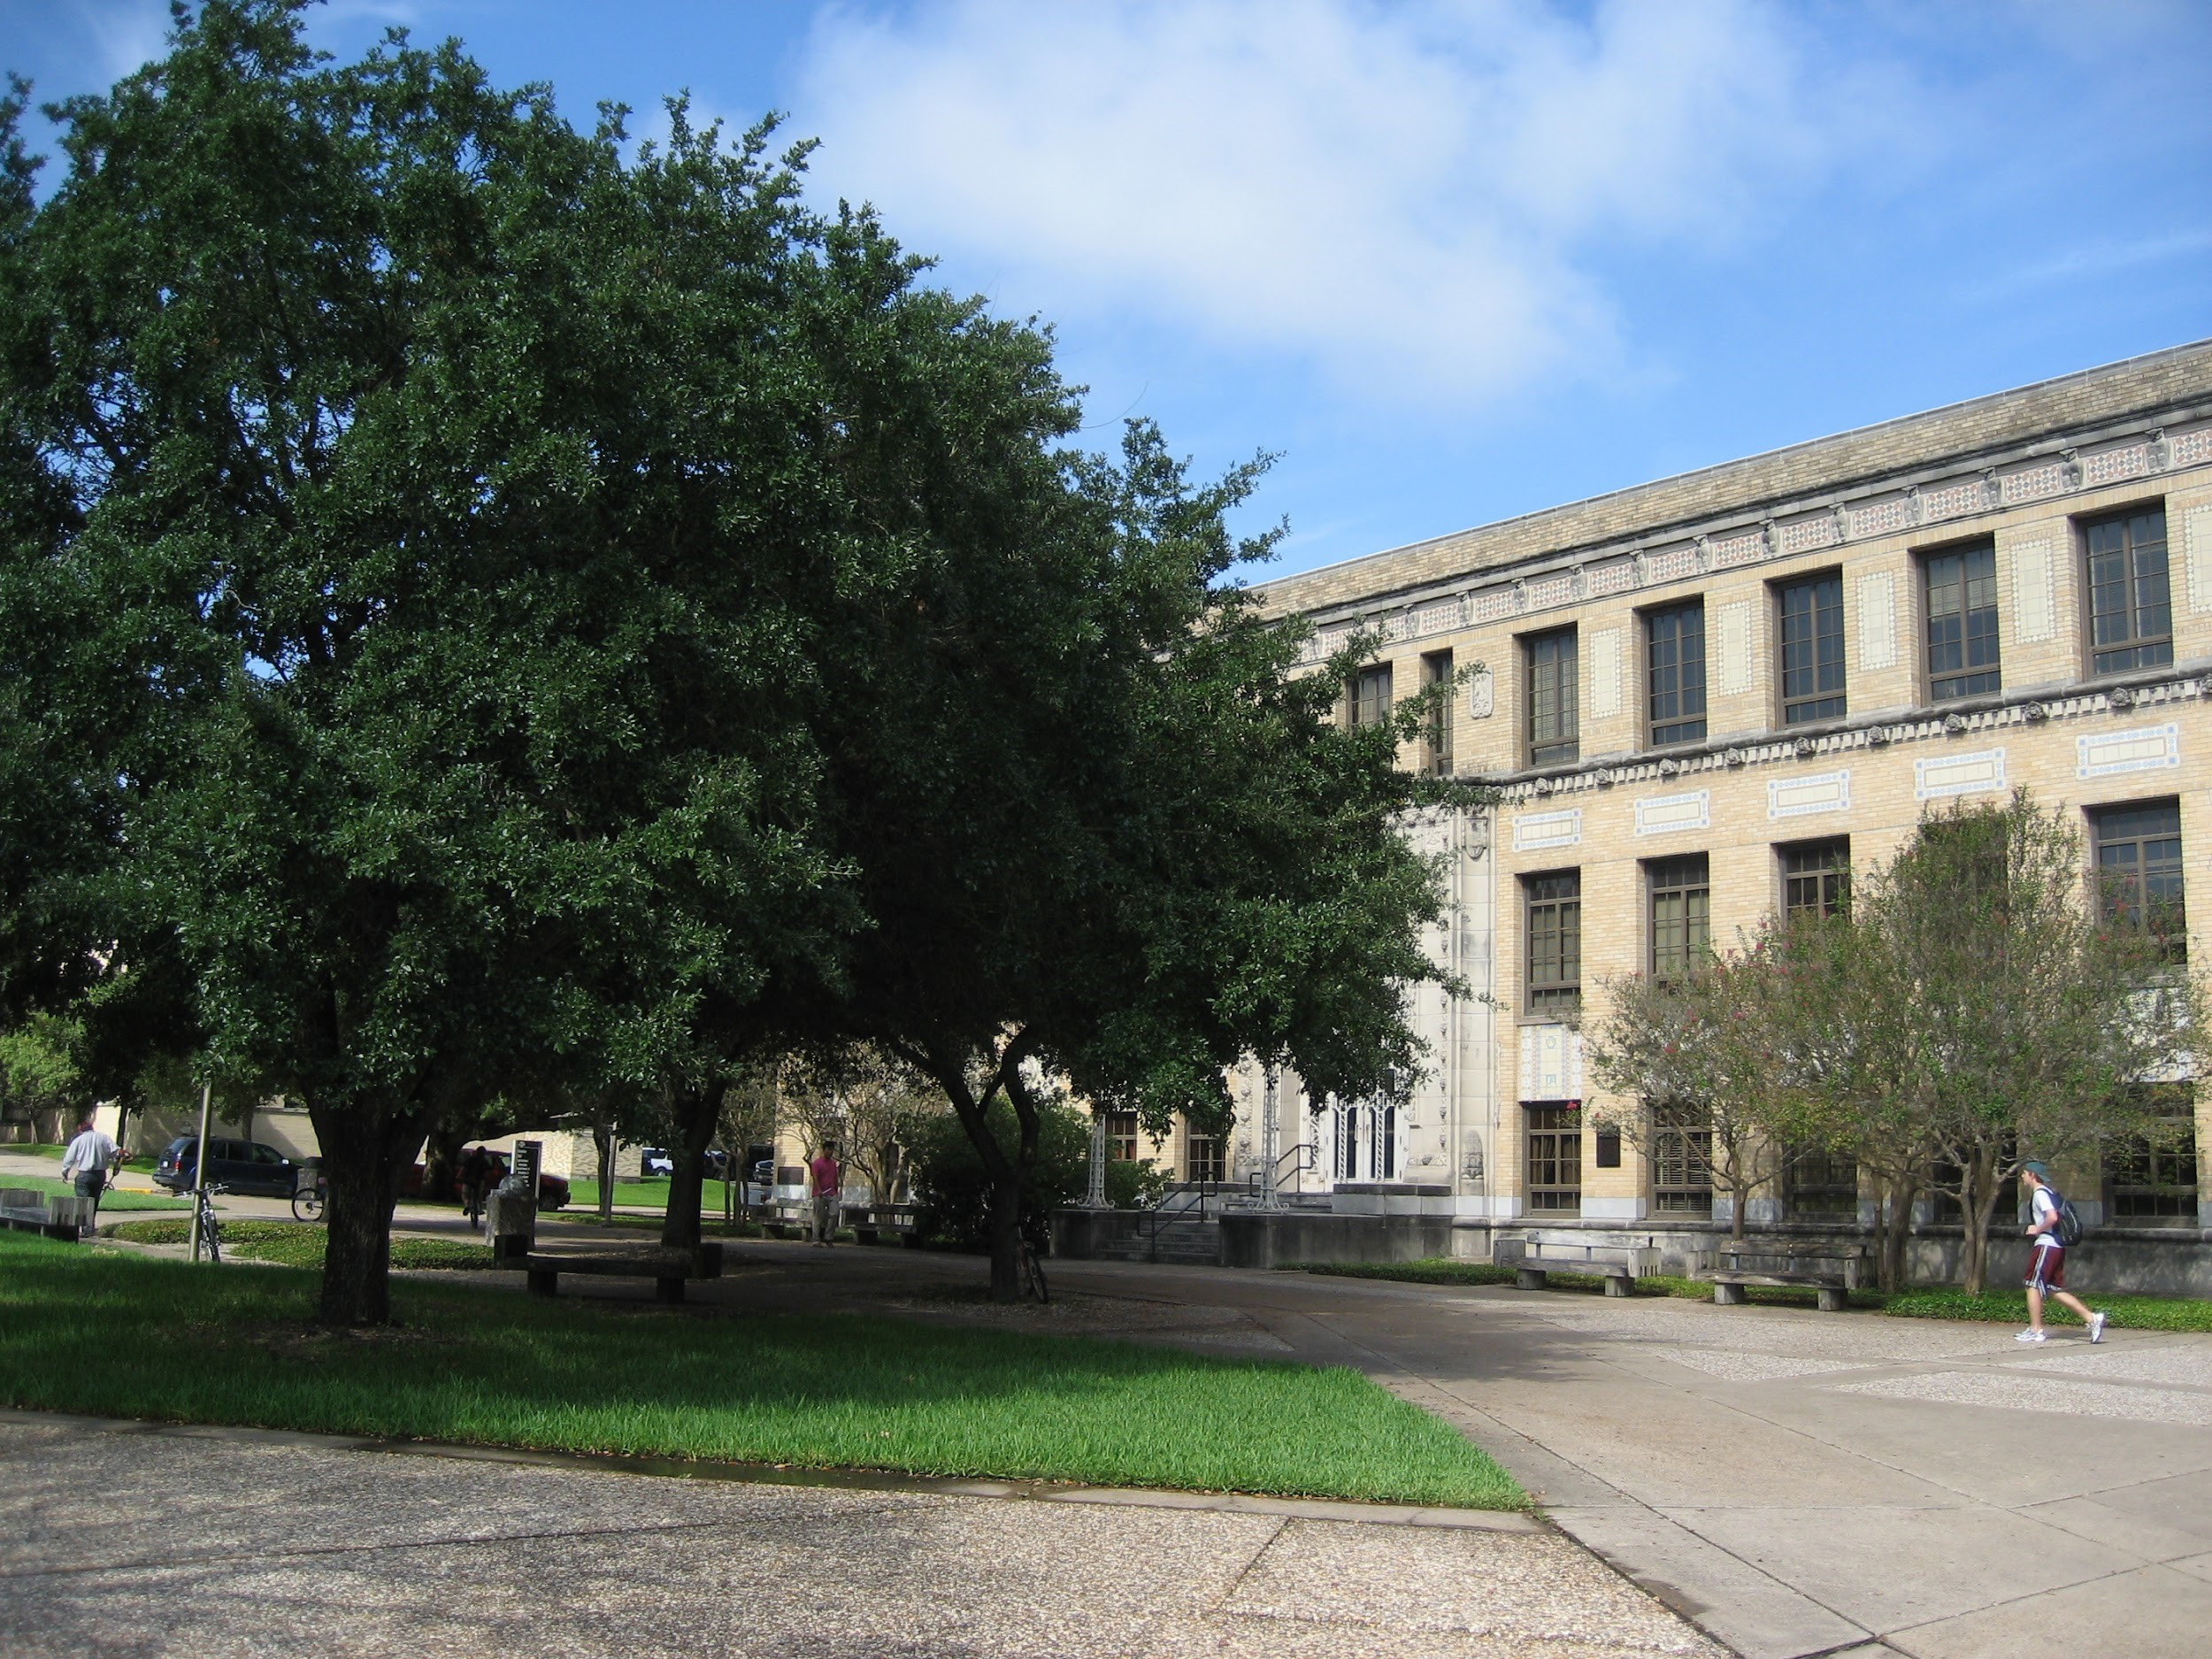
\includegraphics[width=0.49\linewidth]{fig_1.jpg}}
 \subfigure[The original target image(target image space we use for panorama)]{
    \label{fig2} %% label for first subfigure
    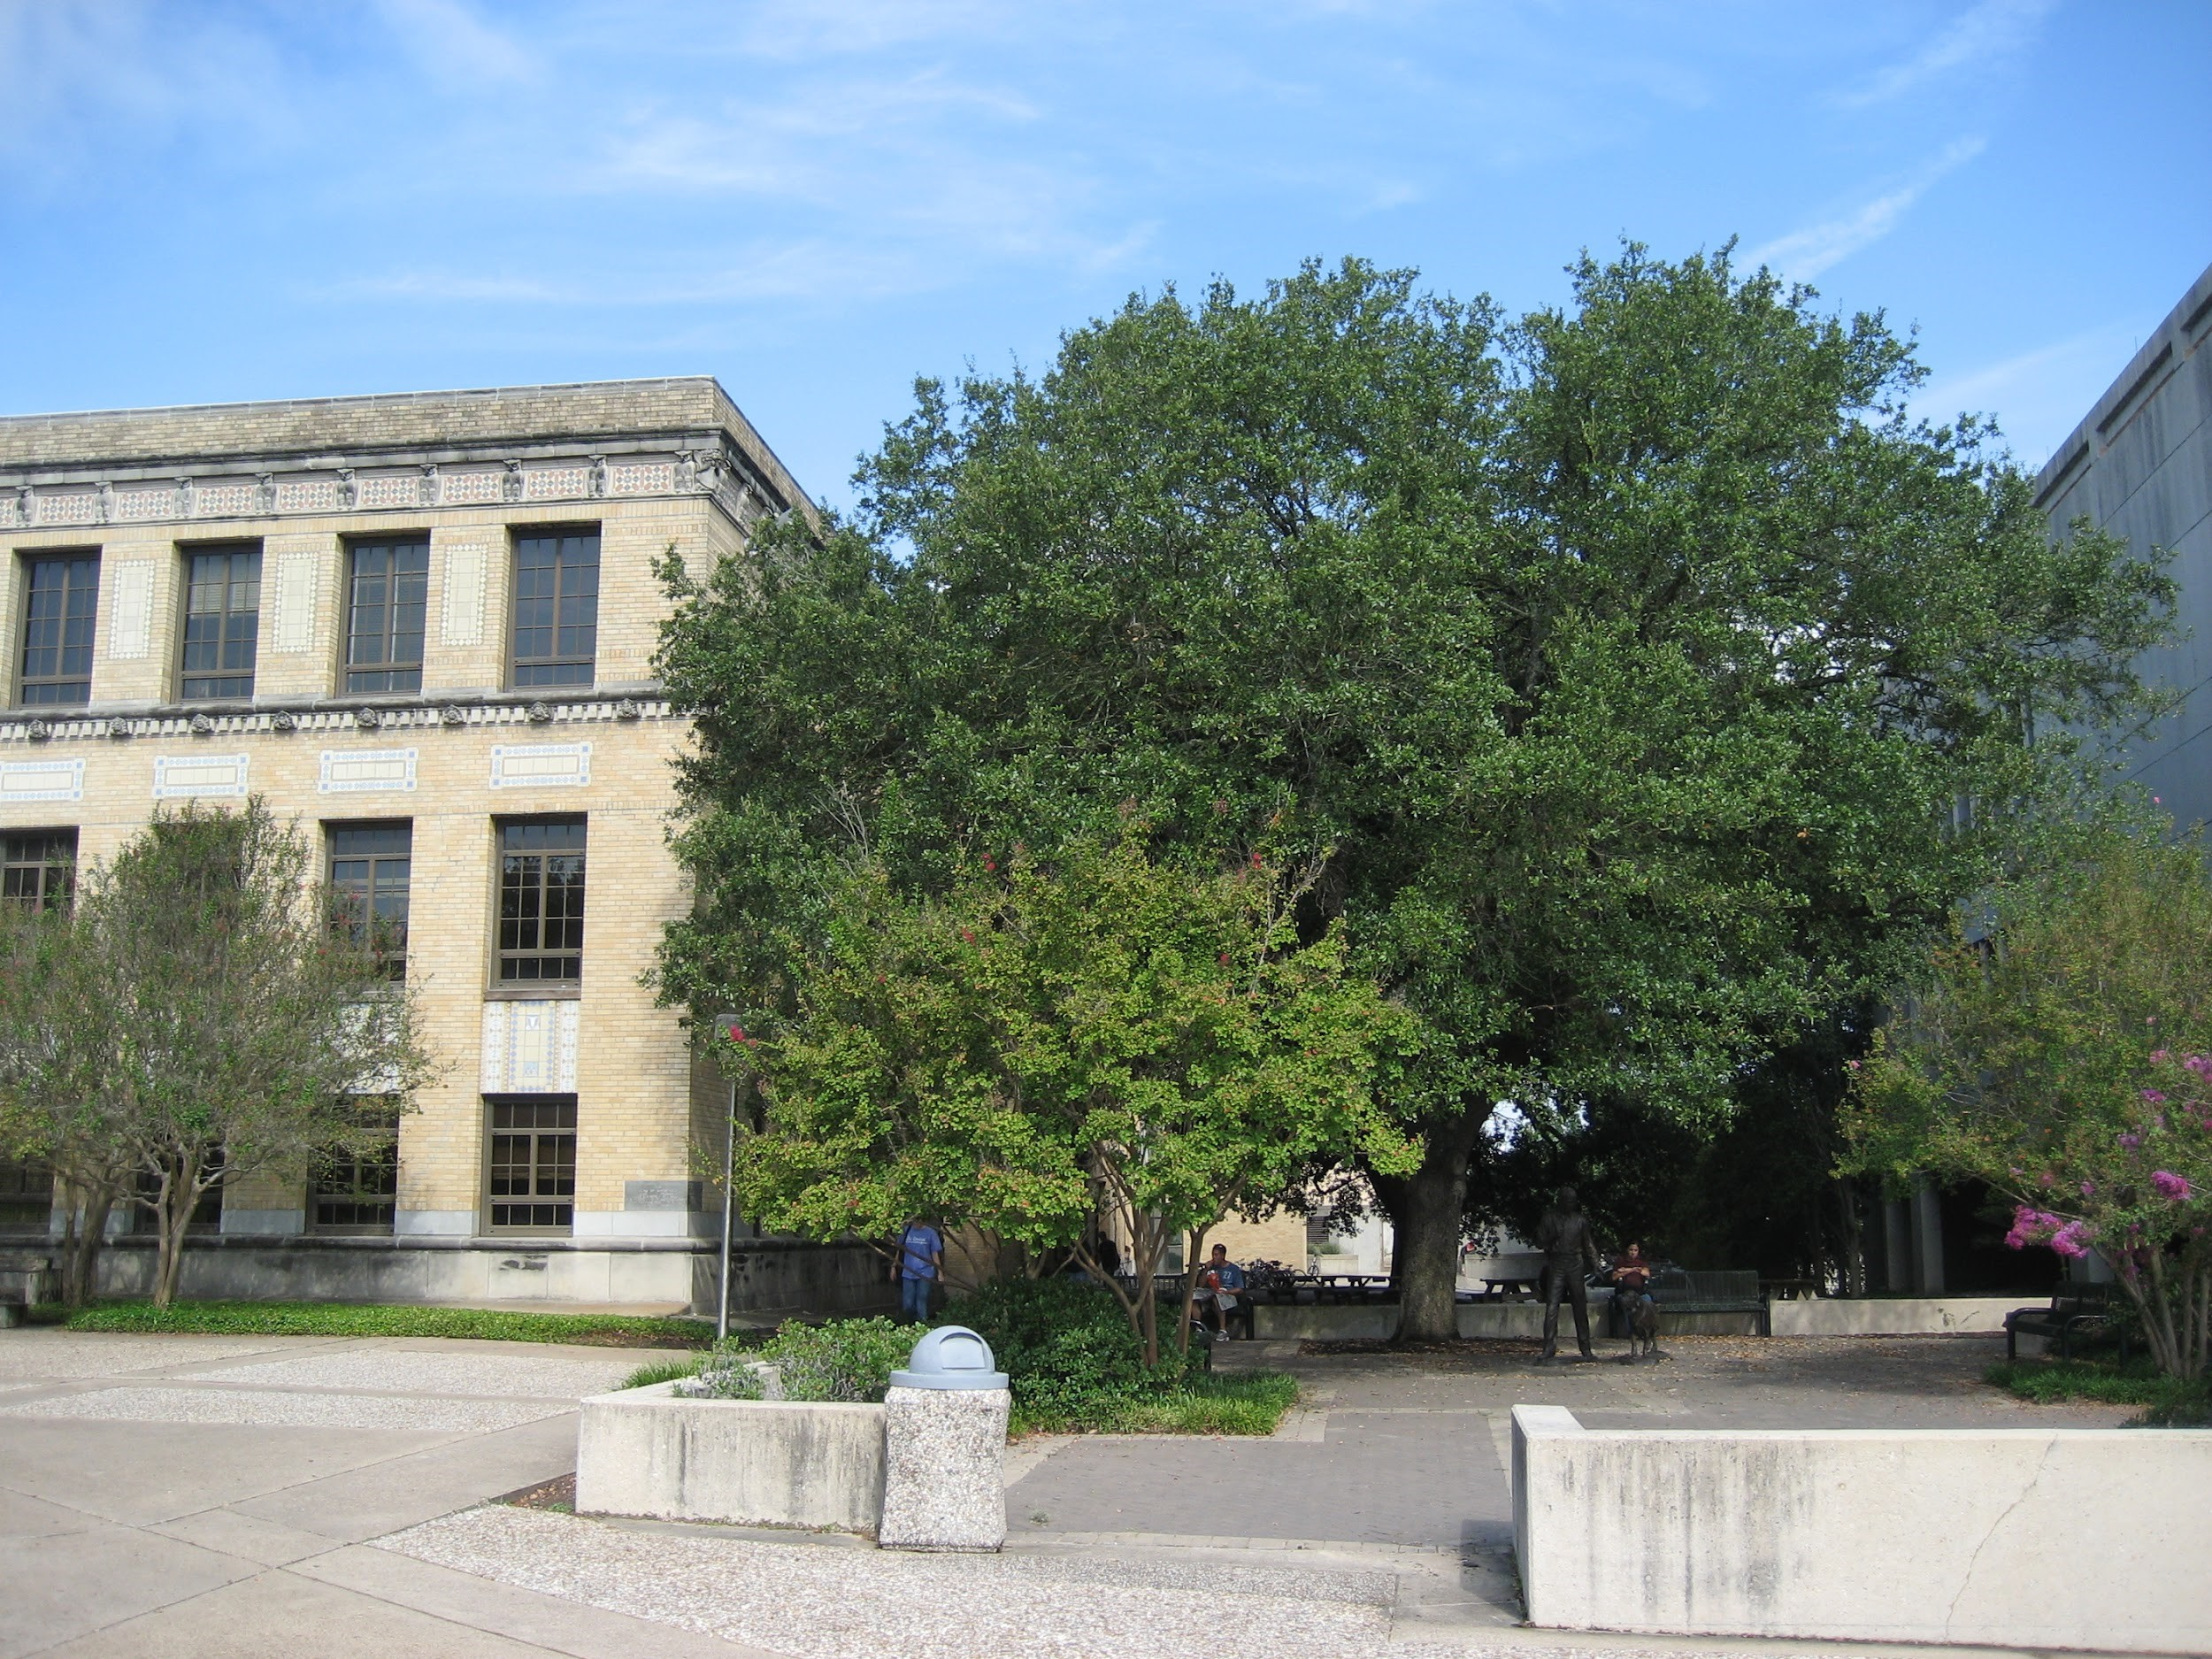
\includegraphics[width=0.49\linewidth]{fig_2.jpg}}
  \caption{Original images}
  \label{org_img} %% label for entire figure
\end{figure*}

\section{Simple DLT Approach}
\subsection{Mathematical Foundation}
In the simplest DLT approach, we first transform the homogeneous equation given in equation 1 as follows:
\begin{equation}
	\mat{x}_i^\prime \times \mat{H}\mat{x}_i = \mat{0}
\end{equation}
Suppose $\mat{H}$ can be decomposed into combination of vectors like:
\begin{equation}
	\mat{H} = \begin{pmatrix}
				\mat{h_1}\\
				\mat{h_2}\\
				\mat{h_3}
		       \end{pmatrix}
\end{equation}
Then we can rewrite equation 2 into the following form:
\begin{equation}
	\mat{H}\mat{x}_i =
	\begin{pmatrix}
		\mat{h}_1\mat{X}_i\\
		\mat{h}_2\mat{X}_i\\
		\mat{h}_3\mat{X}_i
	\end{pmatrix}
\end{equation}
Suppose the coordinates of the set of points we have are:
\begin{equation}
	\begin{split}
		\mat{x}_i^\prime = (x_i^\prime, y_i^\prime, z_i^\prime)\\
		\mat{x}_i = (x_i, y_i, z_i)
	\end{split}
\end{equation}
Then we have:
\begin{equation}
  \mat{x}_i^\prime\times \mat{H}\mat{x}_i =
  \begin{pmatrix}
    y_i^\prime\mat{h}_3\mat{x}_i - z_i^\prime\mat{h}\mat{x}_i\\
	z_i^\prime\mat{h}_1\mat{x}_i - x_i^\prime\mat{h}^3\mat{x}_i\\
	x_i^\prime\mat{h}_2\mat{x}_i - y_i^\prime\mat{h}_1\mat{x}_i
  \end{pmatrix}
\end{equation}
As we have $\mat{h}_i\mat{x}_i = \mat{x}_i^T \mat{h}_j^T$, we can further get the following simultaneous linear equations set:
\begin{equation}
	\begin{bmatrix}
		\mat{0}^T & -z_i^\prime\mat{x}_i^T & y_i^\prime\mat{x}_i^T\\
		z_i^\prime\mat{x}_i^T & \mat{0}^T & -x_i^\prime\mat{x}_i^T\\
		-y_i^\prime\mat{x}_i^T & x_i^\prime\mat{x}_i^T & \mat{0}^T
	\end{bmatrix}
	\begin{pmatrix}
		\mat{h}_1^T\\
		\mat{h}_2^T\\
		\mat{h}_3^T
	\end{pmatrix} = \mat{0}
\end{equation}

Since we can obtain the 3rd row of the left matrix above using by combining first two rows up to scale, we can safely prune equation 7 to only preserve the linearly independent first two rows in that matrix and obtain:
\begin{equation}
	\mat{A}_i
	\mat{h} = \mat{0}
\end{equation}
where
\begin{equation}
	\mat{A} = 
	\begin{bmatrix}
		\mat{0}^T & -z_i^\prime\mat{x}_i^T & y_i^\prime\mat{x}_i^T\\
		z_i^\prime\mat{x}_i^T & \mat{0}^T & -x_i^\prime\mat{x}_i^T
	\end{bmatrix}, 
	\mat{h} = 
	\begin{pmatrix}
		\mat{h}_1^T\\
		\mat{h}_2^T\\
		\mat{h}_3^T
	\end{pmatrix}
\end{equation}
As we know:
\begin{equation}
	\mat{H} = 
	\begin{pmatrix}
		\mat{h}_1\\
		\mat{h}_2\\
		\mat{h}_3
	\end{pmatrix}
	=
	\begin{bmatrix}
		h_1 & h_2 & h_3\\
		h_4 & h_5 & h_6\\
		h_7 & h_8 & h_9
	\end{bmatrix}
\end{equation}

Now we have come to the point that is very similar to what we have done before in Project 1. After dehomogenization, the equation 8 we get is actually a equation with 8 unknowns in $\mat{h}$ (8 DoFs) which we can solve exactly if we have 4 point pairs (every point pair provide 2 equations), to get the homography we can do as the followings:
\begin{itemize}
	\item If we have exact 4 point correspondences in both images, we can solve equation 8 to get an exact solution, but as there might be some noises in both images, it could lead to very bad results.
	\item We can also solve this equation is we can find more point correspondence to get so-called overdetermined solution through singular value decomposition (SVD), that way we should get more accurate results since we are provided with more information in the image.
\end{itemize}


\subsection{Experiment}
In this section we present the setup of our experiment throughout the process of solving all three problems in this project. If without further specification, all experiments we used for problem 1-3 follow the setup here, including the point choices.
\subsubsection{Point Choice}
As we have mentioned before, to acquire better and accurate homography transformation between two images, we should choose point pairs in both images that are not colinear. Following this principle, we choose points in two images as shown in Fig. \ref{pchoice}. The point choices are marked using red and green X markers in two images respectively.
\begin{figure*}[!hbpt]
  \subfigure[Point choices in the first image]{
\label{pchoice-1st} %% label for second subfigure
\includegraphics[width=0.49\linewidth]{pchoice-1st.jpg}}
 \subfigure[Corresponding points in the second image]{
    \label{pchoice-2nd} %% label for first subfigure
    \includegraphics[width=0.49\linewidth]{pchoice-2nd.jpg}}
  \caption{Point pair choices between two original images}
  \label{pchoice} %% label for entire figure
\end{figure*}


\subsubsection{Panorama}
Ideally after we solved $\mat{H}$, we can use simple MATLAB functions to apply the homography on the source image and rectify it to the same space of Fig. \ref{org_img} (b), the result we get at this step is shown in Fig. \ref{dlt1}. Obviously, we are still one step away from the panorama, so how do we combine the new image we get and Fig. \ref{org_img} (b) together? In our approach, we used two MATLAB methods \emph{imref2d} and \emph{imfuse} to do the trick. In MATLAB, \emph{imref2d} function can be used to construct a spatial ref object assuming the world coordinate system is co-aligned with the intrinsic coordinate system while \emph{imfuse} function can leverage the reference info of two images and combine them together as one image. After applying those two methods on our result, we can get the final panorama shown in Fig. \ref{pure_dlt}.

\begin{figure}[htbp]
\begin{center}
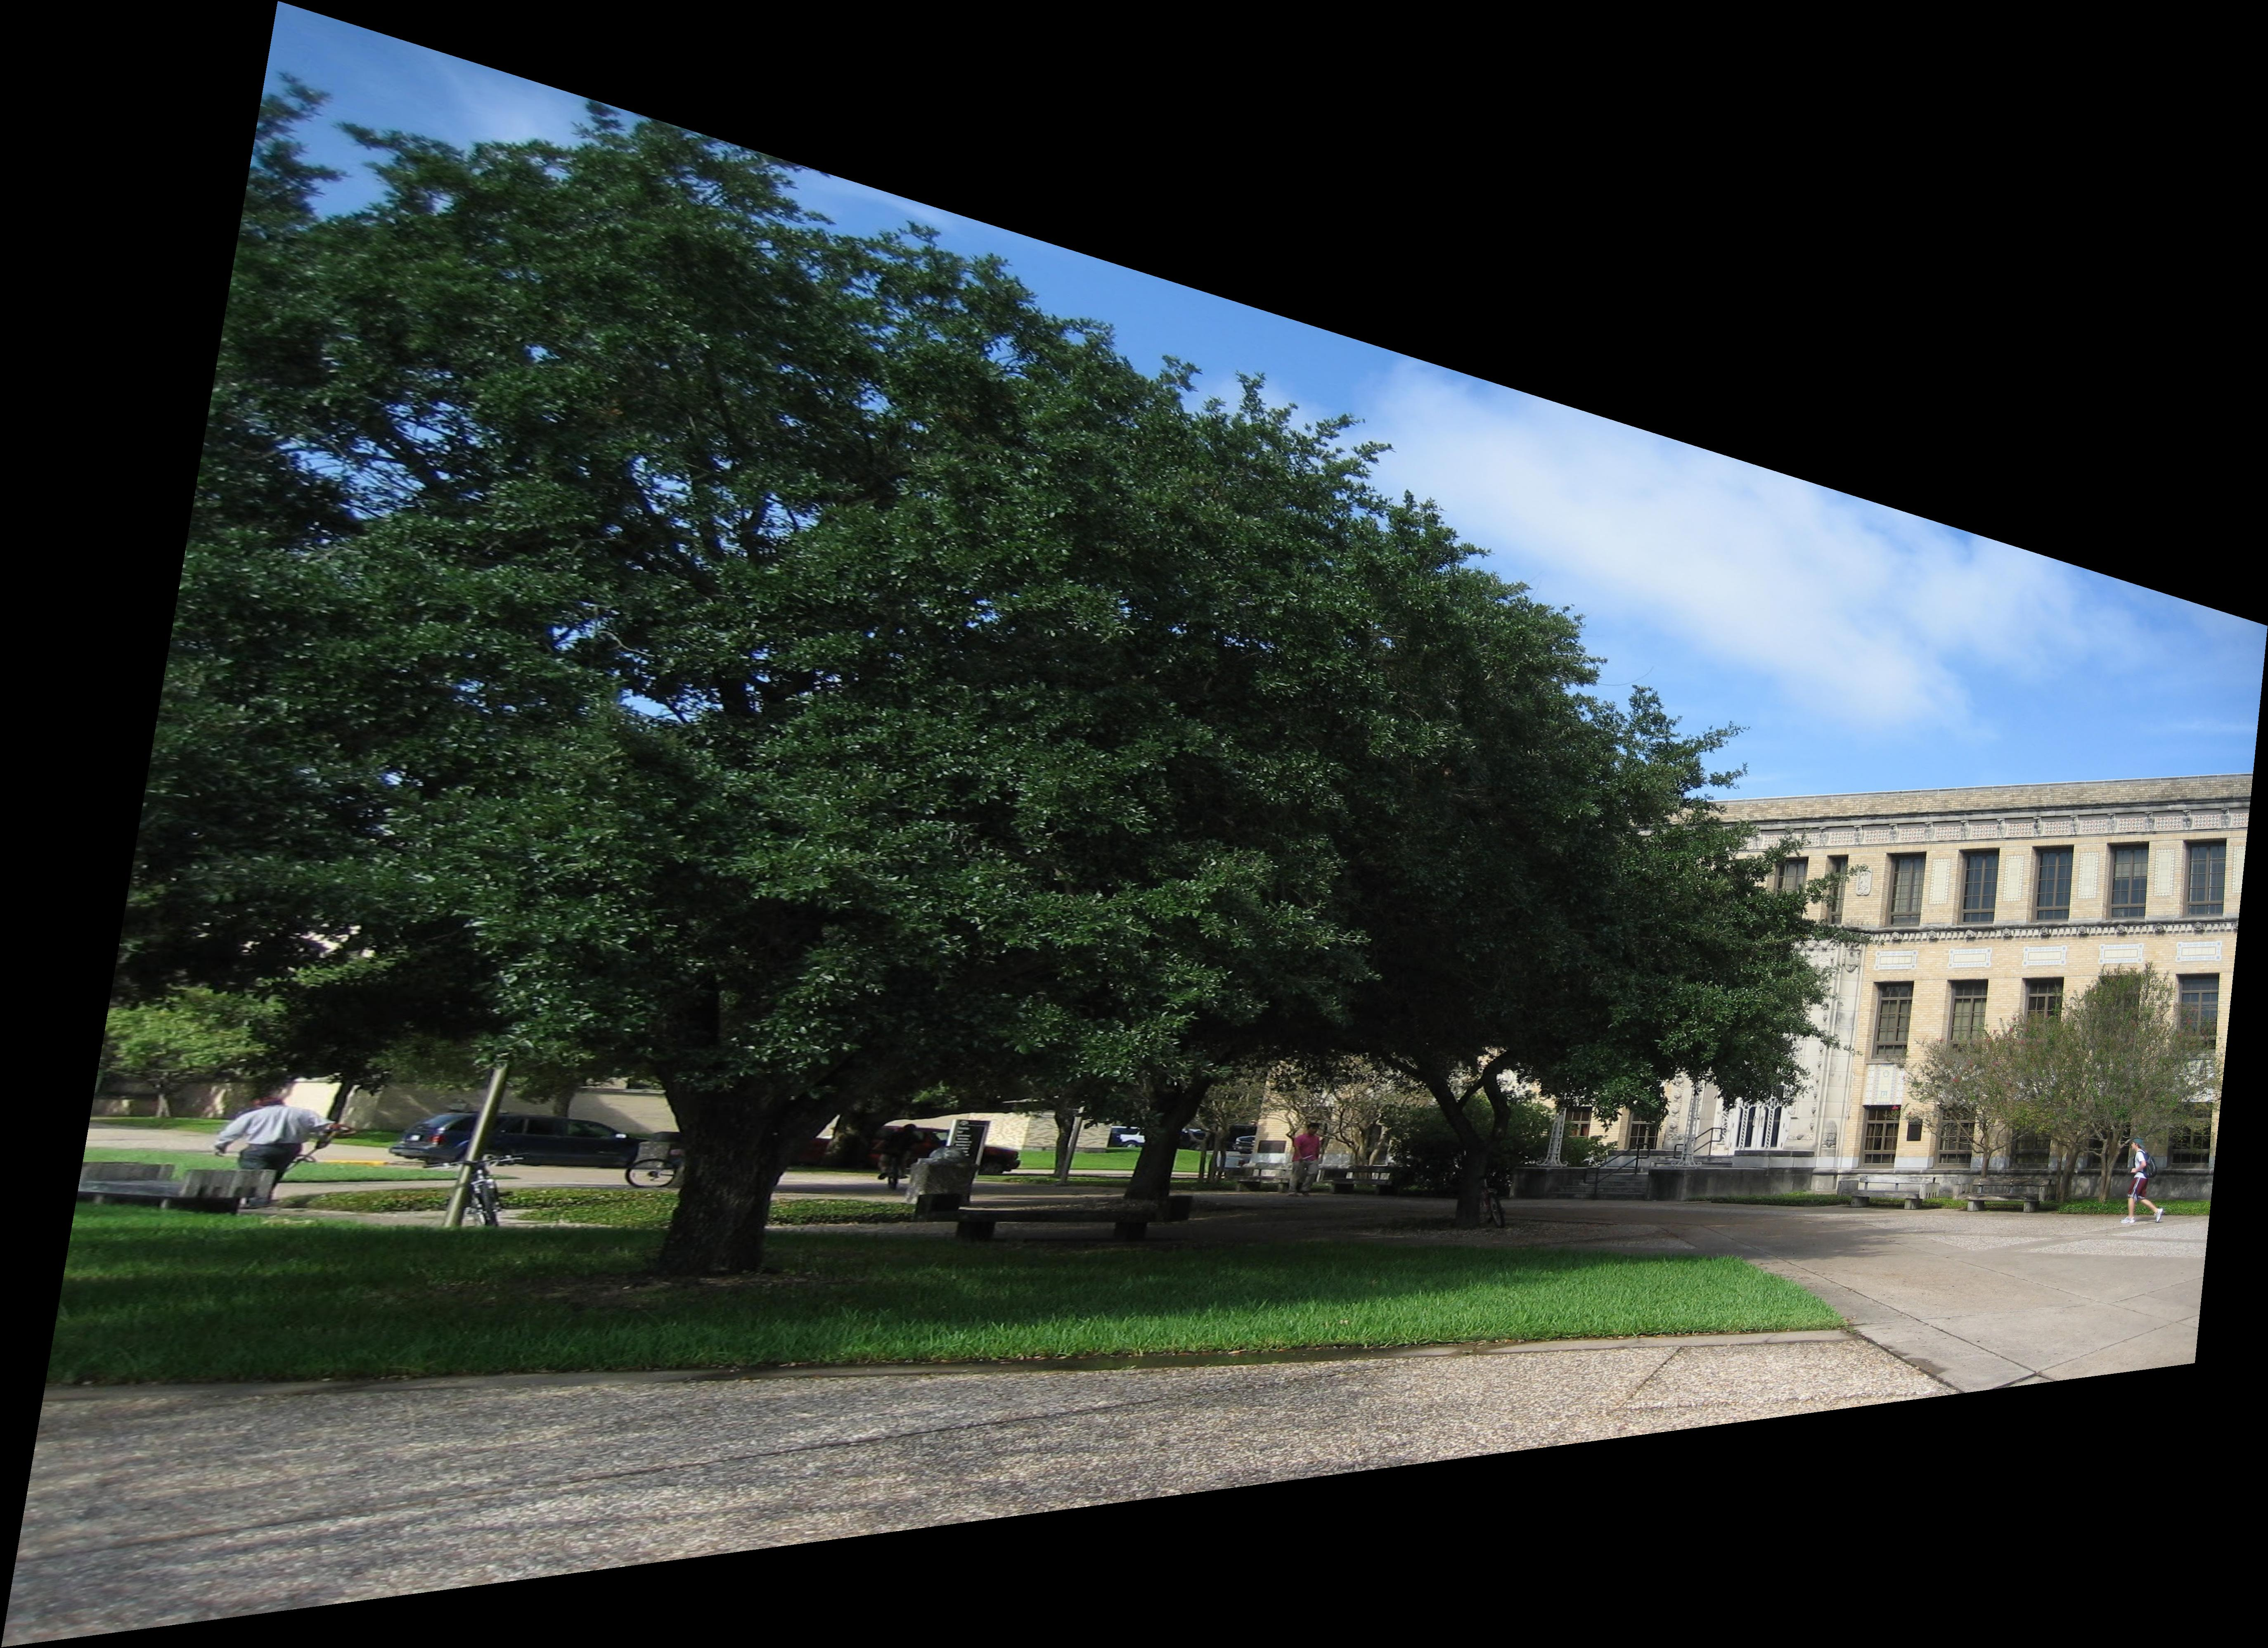
\includegraphics[width=\linewidth]{dlt.jpg} 
\end{center}	   
\caption{The direct result we acquire after applying homography}\label{dlt1}
\end{figure}

\begin{figure}[htbp]
\begin{center}
\includegraphics[width=\linewidth]{pure_dlt.jpg} 
\end{center}	   
\caption{Panorama formed by result of pure DLT}\label{pure_dlt}
\end{figure}

Intuitively in the final panorama, the portion of image that are marked green is the transformed image of Fig. \ref{org_img} (a) while the magneta portion is purely from Fig. \ref{org_img} (b). The portion that are marked as grey is of course the overlapping pixels from both images. As we can see, due to a good choice of point pairs and the high quality of the original photo, the result we got is already considerably accurate.

\subsection{Summary}

\section{Normalized DLT}
As we learn from textbook, the accuracy of result homography generated by pure DLT is relevant on the coordinate frame for expressing points and the best coordinate system for DLT is the normalized system (based on input points). Thus we can improve the result of DLT by first normalizing the input points into a new coordinate system, do DLT algorithm and then denormalize to get an actual homography that can take image to the target space. Through the normalization, we can deal with less well conditioned problems using DLT.
\subsection{Mathmatical Foundation}
The normalization process can be summarized as follows:
\begin{itemize}
	\item Compute a similarity transformation $\mat{T}$, consisting of a translation and scaling that maps $\mat{x}_i$ to $\bar{\mat{x}}_i$ such that the centroid of all points $\bar{\mat{x}_i}$ is the coordinate origin $(0, 0)^T$ and their average distance from the origin is $\sqrt{2}$.
	\item Compute a similar transformation $\mat{T}^\prime$ using the same process to map $\mat{x}_i^\prime$ to $\bar{\mat{x}}_i^\prime$.
	\item Apply simple DLT in Problem 1 using the new corresponding point pairs $\bar{\mat{x}}_i\leftrightarrow \bar{\mat{x}}_i^\prime$ to obtain the normalized homography $\bar{\mat{H}}$
	\item Use $\mat{H} = {\mat{T}^\prime}^{-1}\bar{\mat{H}}\mat{T}$ to denormalize the homography from last step and get the actual homography.
\end{itemize}

Now let's do some math to further clarify the normalization process. Without loss of generality, suppose we wanna find the homography $\mat{T}$ for normalizing an image using a set of points $\mat{x}_i = (x_i, y_i, 1)^T$  in it, where:
\begin{equation}
	T = 
	\begin{pmatrix}
		s & 0 & t_x\\
		0 & s & t_y\\
		0 & 0 & 1
	\end{pmatrix}
\end{equation}

and it consists the combination of both the translation and scaling process that can take $\mat{x}_i$ to a new set of points $\bar{\mat{x}}_i = ({x}_i^\prime, {y}_i^\prime, 1)^T$ so that ${\mat{x}}_i^\prime = \mat{T}\mat{x}_i$, that is to say:
\begin{equation}
	{\mat{x}}_i^\prime = \mat{T}\mat{x}_i = 
	\begin{pmatrix}
		sx_i + t_x\\
		sy_i + t_y\\
		1
	\end{pmatrix}= 
	\begin{pmatrix}
		{x}_i^\prime\\
		{y}_i^\prime\\
		1
	\end{pmatrix}
\end{equation}

Also as we mentioned, the centroid of the point set ${\mat{x}}_i^\prime$ should be $(0, 0)$, which means:
\begin{equation}
	\begin{pmatrix}
		\bar{x^\prime}\\
		\bar{y^\prime}\\
		1
	\end{pmatrix} = 
	\begin{pmatrix}
		s\bar{x} + t_x\\
		x\bar{y} + t_y\\
		1
	\end{pmatrix} = (0, 0, 1)^T
\end{equation}

where $\bar{x}, \bar{y}, \bar{x^\prime}, \bar{y^\prime}$ are the average of coordinates in both sets of points $\mat{x}_i$ and $\mat{y}_i$.

Additionally, we know that the average distance between origin and points in the normalized coordinate system is $\sqrt{2}$, therefore:
\begin{equation}
	\begin{split}
		&\frac{1}{n}\sum _{i}^n\sqrt{{x_i^\prime}^2 + {y_i^\prime}^2}\\
		=&\frac{s}{n}\sum_{i}^n\sqrt{(x_i - \bar{x})^2 + (y_i - \bar{y})^2} = \sqrt{2}
	\end{split}
\end{equation}

which means:
\begin{equation}
	s = \frac{\sqrt{2}}{\frac{1}{n}\sum_i^n\sqrt{(x_i - \bar{x})^2 + (y_i - \bar{y})^2}}
\end{equation}

Now, we can simply apply the point coordinates in certain image into equation 15 to solve $s$ and then apply $s$ into equation 13 to obtain both $t_x$ and $t_y$, thereby the similar normalization transformation homography can be solved for both images we have. Say $\mat{T}$ and $\mat{T}^\prime$ are two such homography for Fig. \ref{org_img} (a) and Fig.\ref{org_img} (b) respectively, and we get two set of normalized coordinates in both images $\hat{\mat{x}}_i, \hat{\mat{x}}_i^\prime$. By applying DLT on normalized point pairs, we obtain the transformation homography between two normalized images to be $\hat{\mat{H}}$. If the actual homography we want is $\mat{H}$, then naturally we have:
\begin{equation}
\begin{split}
	&\mat{x}_i^\prime = \mat{H}\mat{x}_i = {T^\prime}^{-1}\hat{\mat{H}}\hat{\mat{x}}_i = \mat{T^\prime}^{-1}\hat{\mat{H}}\mat{T}\mat{x}_i\\
	\Rightarrow &\mat{H} = {\mat{T}^\prime}^{-1}\hat{\mat{H}}\mat{T}
\end{split}
\end{equation}

So far, we have showed mathematically how we can normalize the image and use the normalized point pairs in DLT obtain the transformation homography between normalized image, as well as how to denormalize the homography back to normal space.

\subsection{Experiment}
As we mentioned in experiment 1, we use the same 20 point pairs as the input of our normalized DLT algorithm and applied the same methodology for imfusing the resulting images together. In this experiment, we still use the DLT approach for finding the homography, the difference here is that we first normalize the point correspondences and use normalized coordinates as the input of DLT. After doing DLT, we denormalize the homography we get and apply it for image synthesis. For brevity we ignored the direct result after applying homography we get from normalized DLT and jump into the Panorama section to show the match between our images:
\begin{figure}[htbp]
\begin{center}
\includegraphics[width=\linewidth]{norm_dlt.jpg} 
\end{center}	   
\caption{Panorama formed by result of normalized DLT}\label{norm_dlt}
\end{figure}

Sadly, due to the high quality of original images and our good choice of point pairs, the pure DLT result is already too good that we cannot notice significant differences caused by applying normalization beforehand. We simply show the result here and leave the discovery of differences in the panorama to the discussion section.

\subsection{Summary}

\section{Gold Standard Algorithm with Sampson Error Function}
Though we noticed pretty good results in both the pure DLT and normalized DLT experiment part, we want to emphasize that this might not be the actual case. As we can easily see from the image we used for experiment, the weather is good and clear, both overall and local lighting condition is promising thus noises in the image are limited. However, in reality, we don't usually have photos as good as these two for computation. When it comes to cloudy, rainy days, or even in the night, there will be a lot of noises in photos taken by cameras. Therefore, both DLT approaches presented above might be led to results with no sense due to noises, we definitely need to take measurement error into consideration in order to deal with varying realistic circumstances. In this section, we present and evaluate the Gold Standard Algorithm (aka MLE) with Sampson Error Function to further improve the robustness of our program.

\subsection{Mathematical Foundation}
Suppose for a given homography $\mat{H}$, without loss of generality we have points in different image spaces $\mat{x} = (x, y), \mat{x}^\prime = (x^\prime, y^\prime)$ that satisfies $\mat{x}^\prime \times \mat{Hx} = 0$. Naturally, this relationship defines an algebraic variety $\emph{V}_H$ in $\mathbb{R}^4$. So if we have a measurement $\mat{x}$ (basically a the measured point by a camera), the vector $\hat{\mat{x}}$ that minimizes the geometric error $\|\mat{x} - \hat{\mat{x}}\|^2$ is the closest point on $V_H$ to $\mat{x}$. From the discussion in the above several sections, we also know that any point $\mat{x} = (x, y, x^\prime, y^\prime)^T$ that lies on $V_H$ will also satisfy equation 8 ($\mat{A}\mat{h} = 0$). We can rewrite equation 8 as $C_H(\mat{x}) = 0$ to emphasize the actual dependency on $\mat{x}$ (once $\mat{h}$ is determined or given, $\mat{A}\mat{h}$ becomes a function of $\mat{x}$). Using Taylor expansion, we have:
\begin{equation}
	C_H(\mat{x} + \delta_{\mat{x}}) = C_H(\mat{x}) + \frac{\partial C_H}{\partial \mat{x}}\delta_{\mat{x}}
\end{equation}
Apparently, in our case, we have $\delta _{\mat{x}} = \hat{\mat{x}} - \mat{x}$ and we desire:
\begin{equation}
	C_H(\hat{\mat{x}}) = 0 \Rightarrow C_H(\mat{x}) + (\frac{\partial C_H}{\partial \mat{x}})\delta \mat{x} = 0
\end{equation}

If we define $J$ as the partial derivative matrix and $\epsilon$ to be the cost $C_H(\mat{x})$ associated with $\mat{x}$, we now turned our original problem into a well-formed minimization problem as:
\begin{itemize}
	\item Find vector $\delta _{\mat{x}}$ that minimizes $\|\delta _{\mat{x}}\|$ subject to $J\delta_{\mat{x}} = -\epsilon$.
\end{itemize}

Using the standard Lagrange multiplier approach for such problem, we can finally get the Sampson error:
\begin{equation}
	\|\delta _{\mat{x}}\|^2 = \delta_{\mat{x}}^T \delta_{\mat{x}} = \epsilon^T(JJ^{T})^{-1}\epsilon
\end{equation}

According to the textbook, when we apply Sampson approximation to geometric distance $d(\mat{x}, C)$ between a point $\mat{x}$ and conic $C$, we have $\epsilon = \mat{x}^TC\mat{x}$ and:
\begin{equation}
	J = \begin{bmatrix}
		\frac{\partial(\mat{x}^TC\mat{x})}{\partial x} & \frac{\partial(\mat{x}^TC\mat{x})}{\partial y}
	\end{bmatrix}
\end{equation}

We can now calculate Jacobian and $\epsilon$ based on point correspondences and plug them in equation 19 to obtain the sampson error.

\subsection{Experiment}
With the DLT approach similar to previous experiment, here we further use the output of DLT as the initial homography and the input to our Gold Standard Algorithm. In our implementation, we build a sampson error function for calculating the sampson error given certain homography (including jacob and epsilon calculation) and then we pass the sampson error function into MATLAB library function \emph{lsqnonlin} which does automatic nonlinear minimization. After the nonlinear library function stops, we got the minimized homography and applied it to combine our images, getting the result shown in Fig. \ref{dlt_min}.
\begin{figure}[htbp]
\begin{center}
\includegraphics[width=\linewidth]{dlt_min.jpg} 
\end{center}	   
\caption{Panorama formed by result of Gold Standard Algo with Sampson Error Function}\label{dlt_min}
\end{figure}

Expectedly, the differences are negligible under human eye especially in such a low resolution, we will combine three results together in discussion for the sake of better comparison. However, we'd like to mention here that the sampson error of different approaches can be summarized as follows:
\begin{table}[!htp]
  \centering
  \caption{Sampson Error for Different Approaches}
  \label{sampson_error}
  \begin{tabular}{ccc}
    \toprule
    pure DLT& normalized DLT & Gold Standard\\
	\midrule
		5.7280 & 5.6887 & 4.5112\\
          \bottomrule
  \end{tabular}
\end{table}

\onecolumn
\section{Discussion}
\begin{figure}[!htbp]
\begin{center}
\includegraphics[width=0.7\linewidth]{pure_dlt.jpg} 
\includegraphics[width=0.7\linewidth]{norm_dlt.jpg}
\includegraphics[width=0.7\linewidth]{dlt_min.jpg} 
\end{center}	   
\caption{Combined result of three approaches (from section 2 to 4)}\label{pure_dlt}
\end{figure}
From the observation, we can find that the pure DLT result stretched the left hand image a little bit
longer and in this case, all the object is longer than it appears in the real world. I inquiried and tested using other points set and found if we choose more coplanar and colinear points, this phenomenon would become even significant than our current settings. The
normalized DLT provide less stretched result, which looks very close to the world plane. And
after Maximum likelihood estimation to reduce geometry error, the image looks even better, and I personally believe even the fidelity and clarity of the panorama seems to be enhanced. I would strongly suggests to use larger pictures like directly opening those 3 image results and quick switch between them, which is perhaps the only way for use to notice the little differences between them.

To wrap up, DLT can help us rectify an image to the space of another image, which can be used to create panorama, but the result produced by it is always worse than the approach of normalized DLT. The reason behind that is that there are unavoidable some noises in camera measurement, and without a normalization the magnitude of errors will be significantly higher. However, by manually identify and choosing point pairs that are accurate and choosing point pairs that are neither coplanar nor colinear, we can reduce the influence of noise in the process. Still, as we learnt from the class, we'd better use DLT to get a init better enough setting and then use other more advanced approach like MLE with sampson error function to further optimize and minimize the measurement error to get a better result in generating the panorama or rectify two images into the same space, or whenever we might need to do some error minimization. Additionally, please be noticed that we attached codes in the appendix for reference, to achieve different settings in different problems, the reader might have to follow instruction comments in code and uncomment or comment some code to get desired functionalities.
\newpage
\appendix

\subsection{Pure DLT}
The $\mat{A}$ matrix constructed using 20 point pairs:
\begin{equation}
\begin{pmatrix}0 & 0 & 0 & -2445.0 & -564.7 & -1.0 & 1.479\cdot 10^6 & 3.415\cdot 10^5 & 604.9\\ 2445.0 & 564.7 & 1.0 & 0 & 0 & 0 & -1.189\cdot 10^6 & -2.745\cdot 10^5 & -486.1\\ 0 & 0 & 0 & -2344.0 & -588.1 & -1.0 & 1.418\cdot 10^6 & 3.557\cdot 10^5 & 604.9\\ 2344.0 & 588.1 & 1.0 & 0 & 0 & 0 & -9.169\cdot 10^5 & -2.301\cdot 10^5 & -391.2\\ 0 & 0 & 0 & -2459.0 & -755.5 & -1.0 & 1.932\cdot 10^6 & 5.936\cdot 10^5 & 785.7\\ 2459.0 & 755.5 & 1.0 & 0 & 0 & 0 & -1.17\cdot 10^6 & -3.596\cdot 10^5 & -475.9\\ 0 & 0 & 0 & -2415.0 & -695.3 & -1.0 & 1.744\cdot 10^6 & 5.02\cdot 10^5 & 722.0\\ 2415.0 & 695.3 & 1.0 & 0 & 0 & 0 & -1.067\cdot 10^6 & -3.073\cdot 10^5 & -442.0\\ 0 & 0 & 0 & -2262.0 & -782.3 & -1.0 & 1.77\cdot 10^6 & 6.12\cdot 10^5 & 782.3\\ 2262.0 & 782.3 & 1.0 & 0 & 0 & 0 & -6.397\cdot 10^5 & -2.212\cdot 10^5 & -282.8\\ 0 & 0 & 0 & -2161.0 & -628.3 & -1.0 & 1.329\cdot 10^6 & 3.863\cdot 10^5 & 614.9\\ 2161.0 & 628.3 & 1.0 & 0 & 0 & 0 & -4.353\cdot 10^5 & -1.266\cdot 10^5 & -201.5\\ 0 & 0 & 0 & -2245.0 & -534.5 & -1.0 & 1.208\cdot 10^6 & 2.875\cdot 10^5 & 537.9\\ 2245.0 & 534.5 & 1.0 & 0 & 0 & 0 & -6.73\cdot 10^5 & -1.602\cdot 10^5 & -299.7\\ 0 & 0 & 0 & -2459.0 & -902.8 & -1.0 & 2.278\cdot 10^6 & 8.363\cdot 10^5 & 926.3\\ 2459.0 & 902.8 & 1.0 & 0 & 0 & 0 & -1.145\cdot 10^6 & -4.205\cdot 10^5 & -465.8\\ 0 & 0 & 0 & -2469.0 & -1060.0 & -1.0 & 2.667\cdot 10^6 & 1.145\cdot 10^6 & 1080.0\\ 2469.0 & 1060.0 & 1.0 & 0 & 0 & 0 & -1.133\cdot 10^6 & -4.866\cdot 10^5 & -459.0\\ 0 & 0 & 0 & -2438.0 & -1345.0 & -1.0 & 3.312\cdot 10^6 & 1.827\cdot 10^6 & 1358.0\\ 2438.0 & 1345.0 & 1.0 & 0 & 0 & 0 & -9.87\cdot 10^5 & -5.443\cdot 10^5 & -404.8\\ 0 & 0 & 0 & -2123.0 & -835.9 & -1.0 & 1.754\cdot 10^6 & 6.903\cdot 10^5 & 825.8\\ 2123.0 & 835.9 & 1.0 & 0 & 0 & 0 & -2.911\cdot 10^5 & -1.146\cdot 10^5 & -137.1\\ 0 & 0 & 0 & -2089.0 & -946.4 & -1.0 & 1.963\cdot 10^6 & 8.893\cdot 10^5 & 939.7\\ 2089.0 & 946.4 & 1.0 & 0 & 0 & 0 & -1.944\cdot 10^5 & -88055.0 & -93.04\\ 0 & 0 & 0 & -2096.0 & -1382.0 & -1.0 & 2.931\cdot 10^6 & 1.932\cdot 10^6 & 1398.0\\ 2096.0 & 1382.0 & 1.0 & 0 & 0 & 0 & -1.098\cdot 10^5 & -72377.0 & -52.38\\ 0 & 0 & 0 & -2215.0 & -1352.0 & -1.0 & 3.016\cdot 10^6 & 1.84\cdot 10^6 & 1362.0\\ 2215.0 & 1352.0 & 1.0 & 0 & 0 & 0 & -3.937\cdot 10^5 & -2.402\cdot 10^5 & -177.8\\ 0 & 0 & 0 & -2235.0 & -1469.0 & -1.0 & 3.305\cdot 10^6 & 2.172\cdot 10^6 & 1479.0\\ 2235.0 & 1469.0 & 1.0 & 0 & 0 & 0 & -4.352\cdot 10^5 & -2.859\cdot 10^5 & -194.7\\ 0 & 0 & 0 & -2052.0 & -688.6 & -1.0 & 1.365\cdot 10^6 & 4.58\cdot 10^5 & 665.1\\ 2052.0 & 688.6 & 1.0 & 0 & 0 & 0 & -1.562\cdot 10^5 & -52400.0 & -76.1\\ 0 & 0 & 0 & -2086.0 & -815.8 & -1.0 & 1.653\cdot 10^6 & 6.464\cdot 10^5 & 792.4\\ 2086.0 & 815.8 & 1.0 & 0 & 0 & 0 & -2.082\cdot 10^5 & -81433.0 & -99.82\\ 0 & 0 & 0 & -2262.0 & -929.6 & -1.0 & 2.111\cdot 10^6 & 8.673\cdot 10^5 & 933.0\\ 2262.0 & 929.6 & 1.0 & 0 & 0 & 0 & -6.091\cdot 10^5 & -2.503\cdot 10^5 & -269.2\\ 0 & 0 & 0 & -2001.0 & -598.2 & -1.0 & 1.117\cdot 10^6 & 3.338\cdot 10^5 & 558.0\\ 2001.0 & 598.2 & 1.0 & 0 & 0 & 0 & -64144.0 & -19177.0 & -32.05\\ 0 & 0 & 0 & -2377.0 & -1231.0 & -1.0 & 2.943\cdot 10^6 & 1.524\cdot 10^6 & 1238.0\\ 2377.0 & 1231.0 & 1.0 & 0 & 0 & 0 & -8.334\cdot 10^5 & -4.315\cdot 10^5 & -350.6 \end{pmatrix}
\end{equation}

The homography we solved out using pure DLT:
\begin{equation}
	\mat{H} = 
	\begin{pmatrix}
		2.214 & -0.2198 & -4239.0\\ 0.6458 & 2.057 & -1435.0\\ 0.0004856 & -2.811\cdot 10^{-5} & 1.0
	\end{pmatrix}
\end{equation}

\subsection{Normalized DLT}
The homographies we used for normalization for both images are as follows: 
\begin{equation}
	\mat{H}_1 = 
	\begin{pmatrix}
		0.004667 & 0 & -10.56\\ 0 & 0.004667 & -4.225\\ 0 & 0 & 1.0
	\end{pmatrix}, 
	\mat{H}_2 = 
	\begin{pmatrix}
		0.004612 & 0 & -1.243\\ 0 & 0.004612 & -4.199\\ 0 & 0 & 1.0
	\end{pmatrix}
\end{equation}

where $\mat{H}_1$ is for Fig. \ref{org_img} (a) and $\mat{H}_2$ for Fig. \ref{org_img} (b).

The $\mat{A}$ matrix constructed using 20 normalized point pairs:
\begin{equation}
\begin{pmatrix}0 & 0 & 0 & -0.8563 & 1.589 & -1.0 & -1.207 & 2.239 & -1.409\\ 0.8563 & -1.589 & 1.0 & 0 & 0 & 0 & -0.8552 & 1.587 & -0.9986\\ 0 & 0 & 0 & -0.3819 & 1.48 & -1.0 & -0.5382 & 2.085 & -1.409\\ 0.3819 & -1.48 & 1.0 & 0 & 0 & 0 & -0.2143 & 0.8303 & -0.5611\\ 0 & 0 & 0 & -0.9196 & 0.6985 & -1.0 & -0.529 & 0.4018 & -0.5752\\ 0.9196 & -0.6985 & 1.0 & 0 & 0 & 0 & -0.8752 & 0.6648 & -0.9518\\ 0 & 0 & 0 & -0.714 & 0.9798 & -1.0 & -0.6202 & 0.8511 & -0.8687\\ 0.714 & -0.9798 & 1.0 & 0 & 0 & 0 & -0.568 & 0.7794 & -0.7955\\ 0 & 0 & 0 & -0.002372 & 0.5735 & -1.0 & -0.001401 & 0.3388 & -0.5907\\ 0.002372 & -0.5735 & 1.0 & 0 & 0 & 0 & -0.0001446 & 0.03495 & -0.06095\\ 0 & 0 & 0 & 0.4721 & 1.292 & -1.0 & 0.6433 & 1.761 & -1.363\\ -0.4721 & -1.292 & 1.0 & 0 & 0 & 0 & -0.1483 & -0.406 & 0.3141\\ 0 & 0 & 0 & 0.0767 & 1.73 & -1.0 & 0.1318 & 2.972 & -1.718\\ -0.0767 & -1.73 & 1.0 & 0 & 0 & 0 & 0.01067 & 0.2406 & -0.1391\\ 0 & 0 & 0 & -0.9196 & 0.01094 & -1.0 & 0.06746 & -0.0008024 & 0.07335\\ 0.9196 & -0.01094 & 1.0 & 0 & 0 & 0 & -0.8321 & 0.009898 & -0.9049\\ 0 & 0 & 0 & -0.967 & -0.7235 & -1.0 & 0.7579 & 0.567 & 0.7837\\ 0.967 & 0.7235 & 1.0 & 0 & 0 & 0 & -0.8448 & -0.6321 & -0.8736\\ 0 & 0 & 0 & -0.8247 & -2.052 & -1.0 & 1.703 & 4.238 & 2.065\\ 0.8247 & 2.052 & 1.0 & 0 & 0 & 0 & -0.5143 & -1.279 & -0.6236\\ 0 & 0 & 0 & 0.646 & 0.3235 & -1.0 & 0.2519 & 0.1261 & -0.3899\\ -0.646 & -0.3235 & 1.0 & 0 & 0 & 0 & -0.3948 & -0.1977 & 0.6111\\ 0 & 0 & 0 & 0.8041 & -0.1922 & -1.0 & -0.1087 & 0.02597 & 0.1351\\ -0.8041 & 0.1922 & 1.0 & 0 & 0 & 0 & -0.6548 & 0.1565 & 0.8142\\ 0 & 0 & 0 & 0.7725 & -2.224 & -1.0 & -1.739 & 5.005 & 2.251\\ -0.7725 & 2.224 & 1.0 & 0 & 0 & 0 & -0.7739 & 2.228 & 1.002\\ 0 & 0 & 0 & 0.219 & -2.083 & -1.0 & -0.4558 & 4.335 & 2.081\\ -0.219 & 2.083 & 1.0 & 0 & 0 & 0 & -0.09276 & 0.8822 & 0.4235\\ 0 & 0 & 0 & 0.1241 & -2.63 & -1.0 & -0.3254 & 6.894 & 2.621\\ -0.1241 & 2.63 & 1.0 & 0 & 0 & 0 & -0.04288 & 0.9083 & 0.3454\\ 0 & 0 & 0 & 0.9781 & 1.011 & -1.0 & 1.106 & 1.144 & -1.131\\ -0.9781 & -1.011 & 1.0 & 0 & 0 & 0 & -0.8728 & -0.9022 & 0.8924\\ 0 & 0 & 0 & 0.82 & 0.4172 & -1.0 & 0.4464 & 0.2271 & -0.5444\\ -0.82 & -0.4172 & 1.0 & 0 & 0 & 0 & -0.642 & -0.3267 & 0.783\\ 0 & 0 & 0 & -0.002372 & -0.1141 & -1.0 & 0.0002473 & 0.01189 & 0.1042\\ 0.002372 & 0.1141 & 1.0 & 0 & 0 & 0 & 3.707\cdot 10^{-6} & 0.0001783 & 0.001563\\ 0 & 0 & 0 & 1.215 & 1.433 & -1.0 & 1.975 & 2.329 & -1.625\\ -1.215 & -1.433 & 1.0 & 0 & 0 & 0 & -1.331 & -1.57 & 1.096\\ 0 & 0 & 0 & -0.5401 & -1.52 & -1.0 & 0.8152 & 2.295 & 1.51\\ 0.5401 & 1.52 & 1.0 & 0 & 0 & 0 & -0.2017 & -0.5679 & -0.3735\end{pmatrix}
\end{equation}

The normalized homography $\mat{H}_{norm}$ we obtained directly by applying DLT to normalized point pairs:
\begin{equation}
	\mat{H}_{norm} = 
	\begin{pmatrix}
		0.004612 & 0 & -1.243\\ 0 & 0.004612 & -4.199\\ 0 & 0 & 1.0
	\end{pmatrix}
\end{equation}

The actual homography $\mat{H}_{denorm}$ (denormalized from $\mat{H}_{norm}$) for rectifying the first image to the space of second one:

\begin{equation}
	\mat{H}_{denorm} = 
	\begin{pmatrix}
		0.9927 & -0.1012 & 0.02453\\ 0.09716 & 0.9928 & 8.025\cdot 10^{-5}\\ 0.04906 & -0.003037 & 1.0
	\end{pmatrix}
\end{equation}

\subsection{Gold Standard Algo with Sampson Error Function}
To begin with, we refer readers to equations 21, 22, 24, 25 for $\mat{A}$ matrix and initial homography $\mat{H}$ we used for gold standard minimization.

After applying the DLT on normalized resulting homography, we get
\begin{equation}
	\mat{H}_{norm} = 
	\begin{pmatrix}
		0.9908 & -0.102 & 0.02453\\ 0.1049 & 0.9977 & 8.43\cdot 10^{-5}\\ 0.6086 & -1.557 & 0.9998
	\end{pmatrix}
\end{equation}

Furthermore, after denormalizing the above homography, we have:

\begin{equation}
	\mat{H}_{denorm} = 
	\begin{pmatrix}
		1.768 & -2.062 & -1858.0\\ 2.692 & -5.607 & -103.7\\ 0.00284 & -0.007267 & 1.154
	\end{pmatrix}
\end{equation}

\newpage
\appendix
\subsection{Main Entry}
\lstinputlisting{codes/hw2.m}
% conference papers do not normally have an appendix


% use section* for acknowledgment





% trigger a \newpage just before the given reference
% number - used to balance the columns on the last page
% adjust value as needed - may need to be readjusted if
% the document is modified later
%\IEEEtriggeratref{8}
% The "triggered" command can be changed if desired:
%\IEEEtriggercmd{\enlargethispage{-5in}}

% references section

% can use a bibliography generated by BibTeX as a .bbl file
% BibTeX documentation can be easily obtained at:
% http://mirror.ctan.org/biblio/bibtex/contrib/doc/
% The IEEEtran BibTeX style support page is at:
% http://www.michaelshell.org/tex/ieeetran/bibtex/
%\bibliographystyle{IEEEtran}
% argument is your BibTeX string definitions and bibliography database(s)
%\bibliography{IEEEabrv,../bib/paper}
%
% <OR> manually copy in the resultant .bbl file
% set second argument of \begin to the number of references
% (used to reserve space for the reference number labels box)
%\bibliographystyle{IEEEtran}
% argument is your BibTeX string definitions and bibliography database(s)
%\bibliography{refs}




% that's all folks
\end{document}


